\documentclass{article}

\input{ddphonism.sty}

\begin{document}
	
	\DsizeMake{0,2,1,3}
	\begin{tikzpicture}[use Hobby shortcut]
	\begin{knot}[
	consider self intersections=true,
	  draft mode=crossings,
	flip crossing/.list={2,4,6}
	]
	\strand ([closed]90:2) foreach \k in {0,2,1,3} { .. (90-360/\theDsize+\k*720/\theDsize:1.5) .. (90+\k*720/\theDsize:2) } (90:2);
	\end{knot}
	\end{tikzpicture}

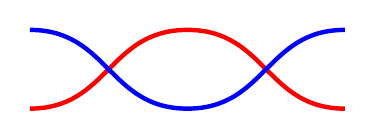
\begin{tikzpicture}
	\draw[red,ultra thick] (0,0) .. controls +(1,0) and +(-1,0) .. (2,1) .. controls +(1,0) and +(-1,0) .. (4,0);
	\draw[blue,ultra thick] (0,1) .. controls +(1,0) and +(-1,0) .. (2,0) .. controls +(1,0) and +(-1,0) .. (4,1);
\end{tikzpicture}

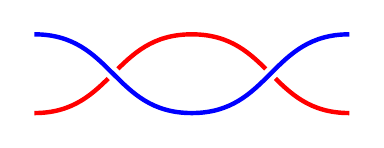
\begin{tikzpicture}
	\draw[red,ultra thick] (0,0) .. controls +(1,0) and +(-1,0) .. (2,1) .. controls +(1,0) and +(-1,0) .. (4,0);
	\draw[white,double=blue,ultra thick,double distance=1.6pt] (0,1)..controls +(1,0) and +(-1,0) .. (2,0) .. controls +(1,0) and +(-1,0) .. (4,1);
\end{tikzpicture}

\begin{tikzpicture}
	\begin{knot}[draft mode=strands]
	\draw[red,ultra thick] (0,0) .. controls +(1,0) and +(-1,0) .. (2,1) .. controls +(1,0) and +(-1,0) .. (4,0);
	\draw[blue,ultra thick] (0,1) .. controls +(1,0) and +(-1,0) .. (2,0) .. controls +(1,0) and +(-1,0) .. (4,1);
	\end{knot}
\end{tikzpicture}

\bigskip\bigskip\bigskip\bigskip\bigskip\bigskip\bigskip\bigskip

\DsizeMake{0,2,1,3,5,4}
\begin{tikzpicture}
	\begin{knot}[draft mode=strands]
	\foreach[count=\nx] \x in {0,2,1,3,5,4} {
		\node (\x) at (\nx*360*2/\theDsize:2){\x};
	}
	\setcounter{Dprev}{4}%
	\foreach[count=\nx] \x in {0,2,1,3,5,4} {
		\draw[red,ultra thick] (\theDprev) .. controls +(\nx*360*2/\theDsize:3) .. (\x);
		\setcounter{Dprev}{\x}%
	}
	\end{knot}
\end{tikzpicture}

\dchords{0,8,6,7,2,4,9,11,1,5,3,10}

0,8,6,7,2,4,9,11,1,5,3,10
	
%	\foreach \x in {#2}{%
%		\ifnum \theDprev=\theDfirst%
%		\draw [style=ddiagramArrow] (\theDprev) -- (\x);%
%		\else \ifnum \theDprev=-1%
%		\else%
%		\draw (\theDprev) -- (\x);%
%		\fi\fi%
%	};%
%	\draw (\theDprev) -- (\theDfirst);%
\end{document}
